\begin{figure}[!ht]
    \centering
    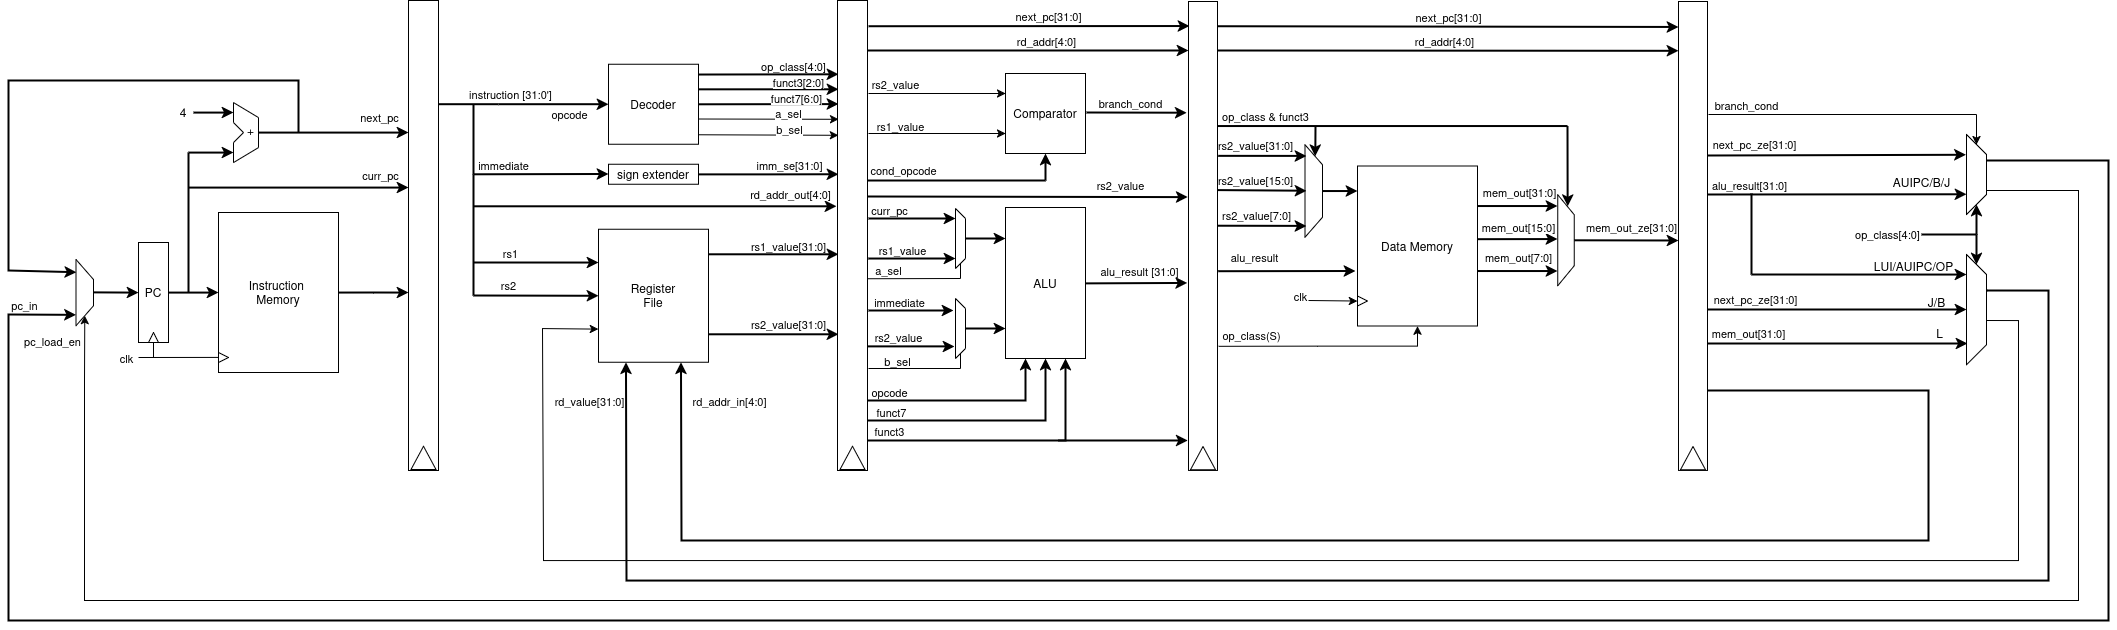
\includegraphics[scale = 0.2]{datapath_pipelined.png}
    \caption{An example of pipelined RISC-V architecture}
    \label{fig:DP_PPL}
\end{figure}

As mentioned earlier, having the processes sensitive to the rising edge of the clock, and having it update output signals after the end is the VHDL equivalent to registers, for example, supposing an input \emph{pc{\_}in} and an output \emph{pc{\_}out}:  

\begin{minted}[fontsize=\footnotesize]{vhdl}
architecture Behavioral of Example is
    signal pc_reg : std_logic_vector(11 downto 0);
begin
process(clk)
    begin
        if rising_edge(clk) then
            pc_reg <= pc_in;
        end if;
    end process;
    pc_out  <= pc_reg;
end Behavioral;
\end{minted}

A process in VHDL executes a routine whenever any signal in the sensitivity list changes, meaning that whatever the routine is, its output is not available until the sensitive inputs change. In the example above \emph{pc{\_}reg} changes only when a rising edge of the clock approaches, thus keeping the output still for the whole clock cycle; The same concept can be applied to all the blocks that compose the architecture, by having all processes clock-sensitive, some kind of pipeline can be naturally implemented.\\
This method, however convenient, does not take into account the signals that are used in multiple process, for example, if \emph{funct3} is passed directly to the DM stage, with \emph{op{\_}class} commanded by a different instruction, the DM could wrongly load or store the result of the original operation.\\
Both for this reason and for not having to change the whole code and thus maintaining clarity over the project's code, the inter-stage registers will be programmed as separate blocks in VHDL. Before starting to code, it is imperative to identify which signals are the ones that need to be passed down and the ones that are not useful anymore. 
From simple analysys of the code, Table \ref{table:signals_pipeline} lists all the outputs expected at the boundary of each stage, indicated as the union of the names of the two stages that the boundary shares.

\begin{table}[ht]
\begin{center}
\begin{tabular}{|c|c|c|c|c|}
    \hline
    IF/ID & ID/IE & IE/DM & DM/WB & WB \\
    \hline
    curr{\_}pc  & curr{\_}pc        & curr{\_}pc        & next{\_}pc        & pc{\_}out \\
    next{\_}pc  & next{\_}pc        & next{\_}pc        & mem{\_}out        & rd{\_}value \\
    instr       & op{\_}class       & op{\_}class       & branch{\_}cond    & pc{\_}load{\_}en\\
                & funct3            & funct3            & alu{\_}result     & mem{\_}we\\
                & funct7            & alu{\_}result     & rd{\_}addr        & rd{\_}addr\\
                & a{\_}sel          & branch{\_}cond    & op{\_}class       & \\
                & b{\_}sel          & rs2{\_}value      &                   & \\
                & imm{\_}se         & rd{\_}addr        &                   & \\
                & rs1{\_}value      &                   &                   & \\
                & rs2{\_}value      &                   &                   & \\
                & rd{\_}addr        &                   &                   & \\
                & cond{\_}opcode    &                   &                   & \\
    \hline
\end{tabular}
\caption{List of input signals for each register}
\label{table:signals_pipeline}
\end{center}
\end{table}

Once that each register is described, not timing requirements for setting the load enable for both destination register and Program Counter is needed, since the change in the IF's input can be updated every clock cycle without any risk of glitching due to the simulation not taking into account the delay of each stage. 
Before setting up the Structural definition of the datapath, including registers and major blocks, the IF stage must be edited to increment the PC before the first register, otherwise PC+4 would instead be returned by the WB, 4 clock cycle after the instruction is first withdrawed from the IM. With this being said, WB will return a value for the PC only during jumps and branches, while the IF will select between PC+4 and the returning value from WB.

\begin{figure}[!ht]
    \centering
    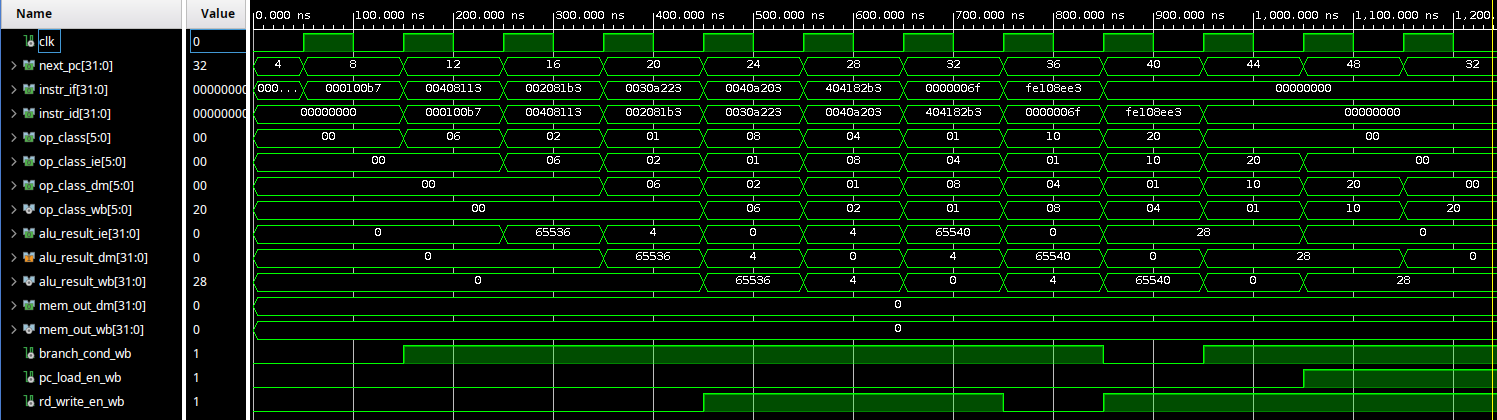
\includegraphics[scale = 0.3]{DPPPL_sim.png}
    \caption{Datapath simulation with pipeline}
    \label{fig:DPPPL_sim}
\end{figure}

Now the processor can execute a part of the instruction in a clock cycle, allowing for higher clock speeds, yet this improvement creates some bugs, one of which can be directly observed from Figure \ref{fig:DPPPL_sim}; In fact, right after the second instruction reaches the execution stage, the \emph{addi} retrieves a 0 instead of 65535 as content of x1, as happens in Figure \ref{fig:WB_sim} where the instruction returns 65540 as a result.
Also, in case of jumps and branches, the correct value for the Program Counter is updated after one clock cycles while the previous instructions still get executed. In addition, since x1 is updated only after 5 clock cycles, the store and load instrucction will operate with different addresses.
While the architecture is now completed, it misses some important features that solve these types of hazards and therefore ensure correct program execution; Thus it becomes essential to implement mechanisms that can handle such hazards to preserve instruction accuracy and consistency while maintaining the performance of a pipelined architecture.  